\documentclass{beamer}
  \usepackage[utf8]{inputenc}
  \usetheme{Warsaw}
  \graphicspath{images/}
  \usepackage{amsmath} 
  \usepackage{amssymb}
  \title{SEC313 : Développement d'applications sécurisées - CTF}
  \author{UFR des Sciences Versailles - M2 SeCReTS}
  \institute{AYOUB Pierre \& CAUMES Clément \& \\ DEBROUASSE Kevin \& Mehdi MTALSI-MERIMI}
  \date{110-broadcast-rsa-2 \\ 113-reversing-2 \\ 122-nfs-and-remote-attack}
  \begin{document}

  \begin{frame}
  \titlepage
  \end{frame}

	\section{110-broadcast-rsa-2}
	
	\subsection{Introduction}
	
	\begin{frame}
	\begin{block}{Ce qu'on connaît} 
		\begin{itemize}
			\setbeamertemplate{itemize item}[circle]
			\item Alice veut envoyer 1 même message à Bob, Charlie et Damien
			\item Bob, Charlie et Damien ont chacun une paire de clés asymétrique RSA et Alice connaît leurs clés publiques
			\item Alice chiffre le message avec un algorithme symétrique et chiffre la clé symétrique avec les clés publiques des 3 destinataires
		\end{itemize}
	\end{block}
	
	\begin{block}{Ce qu'on possède} 
		\begin{itemize}
			\setbeamertemplate{itemize item}[circle]
			\item 1 fichier chiffré \textbf{ciphertext.bin}
			\item 3 fichiers chiffrés \textbf{enveloppe1.bin}, \textbf{enveloppe2.bin} et \textbf{enveloppe3.bin}
			\item 3 clés publiques \textbf{pubkey1.pem}, \textbf{pubkey2.pem} et \textbf{pubkey3.pem}
		\end{itemize}
	\end{block}
	
    \end{frame}
	
	\subsection{Description de la problématique}
	
	\begin{frame}
	\begin{block}{Ce que l'on cherche}
		\begin{itemize}
		\item Nous sommes Oscar et nous voulons connaître le contenu du message envoyé par Alice
		\end{itemize}
	\end{block}
	\begin{block}{Comment réussir l'attaque?}
		\begin{itemize}
		\item Trouver un moyen de calculer la clé symétrique en attaquant l'algorithme RSA (étape 1)
		\item Déchiffrer le message initial avec la clé symétrique qui vient d'être calculée (étape 2)
		\end{itemize}
	\end{block}
    \end{frame}
	
	\subsection{Méthode générale de résolution}
    \begin{frame}
	\begin{block}{Etape 1.1}
		\begin{itemize}
		\item Interpréter les 3 clés publiques utilisés pour chiffrer la clé symétrique choisi par Alice. Ces clés sont écrites sous le format \textbf{PEM} et sont codés en Base64. On obtiendra \textbf{n} et \textbf{e}. 
		\end{itemize}
	\end{block}
	\begin{exampleblock}{Application au problème} 
		Les trois destinataires possède le même \textbf{n}!
	\end{exampleblock}
	\end{frame}
	\begin{frame}
	\begin{block}{Etape 1.2}
		\begin{itemize}
			\item Interpréter les 3 enveloppes qui sont le résultat du chiffrement asymétrique avec les 3 clés publiques des destinataires. On doit donc traduire les octets en entier.
		\end{itemize}
	\end{block}

	\begin{exampleblock}{Application au problème} 
		Le chiffrement asymétrique RSA correspond à : $c \equiv m^e [n]$ \\
		On obtient donc mathématiquement :
		\begin{itemize}
			\item $c_1 \equiv m^3$ $mod$ $n_1 \Leftrightarrow m^3 \equiv c_1$ $mod$ $n_1$
			\item $c_2 \equiv m^3$ $mod$ $n_2\Leftrightarrow m^3 \equiv c_2$ $mod$ $n_2$
			\item $c_3 \equiv m^3$ $mod$ $n_3\Leftrightarrow m^3 \equiv c_3$ $mod$ $n_3$
		\end{itemize}
		(avec $c_i$ l'enveloppe $i$, $e=3$ l'exposant publique des destinataires utilisé par Alice et $n_i$ le module du destinataire $i$).
	\end{exampleblock}
	\end{frame}
	\begin{frame}
		\begin{block}{Etape 1.3}
			\begin{itemize}
				\item Par l'application du théorème des restes chinois, on trouve $m^3$.
				\item Sachant que les exposants publiques choisis par les destinataires sont très petits (ici $3$), on peut facilement calculer la racine cubique de $m^3$ et ainsi trouver $m$.
				\item $m$ (qui est en réalité un nombre) est maintenant traduit en octets car c'est un message texte. 
			\end{itemize}
		\end{block}
		\begin{exampleblock}{Application au problème} 
			On obtient donc $m$ : 
			
			\tiny{Are we there yet?\\
				--------------     Almost there!      -----------------\\
				filename: ciphertext.bin\\
				cipher: camellia-256-ofb\\
				key: EAEC5BA147E9C823C64CC9914D13779979D255E5CF615EA89789C564768FCB3A\\
				iv: 9E20C0E3D433BFF7F37ECC7B74091EF8\\}
		\end{exampleblock}
    \end{frame}

	\begin{frame}
		\begin{block}{Etape 2}
			Les enveloppes envoyées par Alice contenait le nom du chiffrement (Camellia), le mode opératoire (OFB), la clé 256 bits et le vecteur d'initialisation. \newline
			On peut donc déchiffrer \textbf{ciphertext.bin} qui est en réalité un fichier HTML contenant le flag. 
		\end{block}
		\begin{center}
		
\includegraphics[scale=0.6]{./110-broadcast-rsa-2.PNG}
		\end{center}
	\end{frame}
	
	\subsection{Détails sur la résolution}
	
	\begin{frame}{Hastad's broadcast attack}
		L'attaque réalisée est l'\textbf{attaque broadcast de Hastad}. Elle est rendue possible par le fait que Alice a envoyé le même message à 3 destinataires différents et qui possèdent un exposant de chiffrement petit (ici $3$). Il met en jeu le \textbf{théorème des restes chinois} et le calcul d'une \textbf{racine cubique}. 
	\end{frame}

	\begin{frame}{Théorème des restes chinois}
		\begin{block}{Théorème}
				L'inconnu est $x$ et nous avons les équations suivantes :
				\begin{itemize}
				\item $x \equiv a_1$ $mod$ $m_1$
				\item $x \equiv a_2$ $mod$ $m_2$
				\item $x \equiv a_3$ $mod$ $m_3$
				Si $m_i$ et $m_j$ premiers deux à deux alors on peut calculer : \newline
				\color{red}$x \equiv \sum \limits_{i=0}^{n}a_i \times M_i \times N_i$ $mod$ $M$ \color{black}
				
				avec $M_i=M / m_{i}$ et $N_i = Mi^{-1}$ $mod$ $m_i$
			\end{itemize}
		\end{block}
	\end{frame}

	\begin{frame}{Théorème des restes chinois}
	\begin{alertblock}{Démonstration pour comprendre l'attaque - Partie 1}
		\begin{itemize}
		\item Pour chaque $i$ les entiers $m_i$ et $M_i=M/m_i$ sont premiers entre eux.
		\item Avec l'algorithme d'Euclide étendu, on a deux coefficients de Bézout $u_i$ et $N_i$ tels que : 
		$u_i\times m_i + N_i\times M_i = 1$ \newline $\Leftrightarrow N_i \times M_i = 1 - u_i \times m_i$ \newline $\Leftrightarrow N_i \times M_i \equiv 1$ $mod$ $m_i$ $et$ $N_i \times M_i \equiv 0$ $mod$ $m_j$
		\item Or, on a : $x \equiv a_i \times N_i \times M_i$ $mod$ $m_i$ \newline $\Leftrightarrow x \equiv a_i \times (1 - u_i \times m_i)$ $mod$ $m_i$ \newline
		$\Leftrightarrow x \equiv a_i \times 1$ $mod$ $m_i$ \newline
		$\Leftrightarrow x \equiv a_i$ $mod$ $m_i$
		\end{itemize}
	\end{alertblock}
	\end{frame}

	\begin{frame}{Théorème des restes chinois}
	\begin{alertblock}{Démonstration pour comprendre l'attaque - Partie 2}
	\begin{itemize}
		\item Supposons que $x'$ est également une solution.
		Donc, on a : \newline $x \equiv a_i \equiv x'$ $mod$ $m_i$
		$\Leftrightarrow m_i | (x-x')$
		\item Comme $m_i$ et $m_j$ sont premiers entre eux, alors $x \equiv x'$ $mod$ $M$
		\item Donc : $x \equiv \sum \limits_{i=0}^{n}a_i \times M_i \times N_i$ $mod$ $M$
		\item On pouvait donc bien utiliser ce théorème pour résoudre notre problème initial et trouver $m^3$
	\end{itemize}
	\end{alertblock}
	\end{frame}
	
	\subsection{Ouverture}
	
	\begin{frame}
	\begin{block}{Comment éviter cette attaque?}
		\begin{itemize}
			\item Arrêter d'envoyer le même message à plusieurs différentes? Difficile à mettre en place
			\item Insérer de l'aléatoire pour que chaque destinataire reçoive un message différent : PKCS\#1 v1.5
		\end{itemize}
	\end{block}
	\begin{exampleblock}{PKCS\#1 v1.5}
	$C=(\mu(M))^e$ $mod$ $n$ avec 
	$\mu(M)=\O\O\O2||r||\O\O||M$ \newline dont $r$ est une valeur aléatoire d'au moins 8 octets
	\end{exampleblock}
	\end{frame}

	\section{113-reversing-2}
	\subsection{Introduction}
	
	\begin{frame}
	
	\begin{block}{Ce qu'on possède} 
		\begin{itemize}
			\setbeamertemplate{itemize item}[circle]
			\item 1 fichier exécutable \textbf{textflag}
		\end{itemize}
	\end{block}

	\begin{block}{Ce qu'on connaît} 
	\begin{itemize}
		\setbeamertemplate{itemize item}[circle]
		\item Cet exécutable s'exécute avec une chaine de caractères en argument qui correspond au mot de passe (flag) à trouver : $./testflag$ $password$
	\end{itemize}
	\end{block}
	
	\end{frame}

	\subsection{Description de la problématique}
	
	\begin{frame}
	\begin{block}{Ce que l'on cherche}
		\begin{itemize}
			\item Nous voulons connaître le mot de passe permettant d'afficher $Welcome!$ 
		\end{itemize}
	\end{block}
	\begin{block}{Comment réussir l'attaque?}
		\begin{itemize}
			\item Faire du reverse engineering afin de trouver quel mot de passe est valide
		\end{itemize}
	\end{block}
	\end{frame}

	\subsection{Méthode générale de résolution}
	\begin{frame}
	\begin{block}{Etape 1}
		\begin{itemize}
			\item Le premier réflexe est de tester le programme en utilisant le débugger \textbf{gdb}
		\end{itemize}
	\end{block}
	\begin{exampleblock}{Détection de gdb et arrêt direct du programme} 
		\begin{center}
			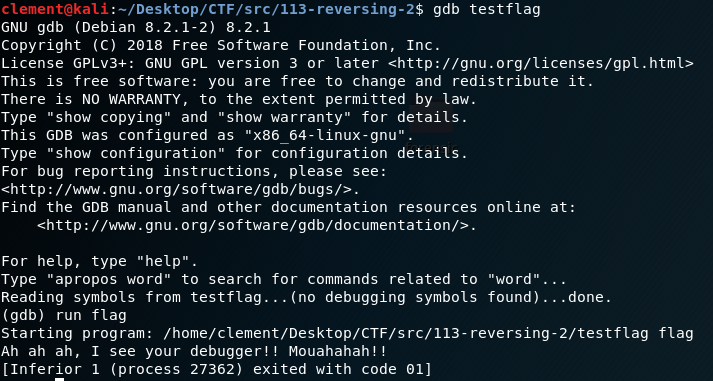
\includegraphics[scale=0.45]{./113-reversing-2-gdb-1.PNG}
		\end{center}
	\end{exampleblock}
	\end{frame}

	\begin{frame}
	\begin{block}{Etape 2}
		\begin{itemize}
			\item Utilisons le désassembleur \textbf{IDA}
		\end{itemize}
	\end{block}
	\begin{exampleblock}{Remarques de l'étude sur IDA} 
		En observant le graphe de flot d'exécution, on arrive à distinguer les différents branchements : 
		\begin{itemize}
			\item il y a le branchement de test qui arrête le programme et affiche "I see your debugger!" (notamment avec la fonction \textbf{ptrace})
			\item il y a également le bloc "Welcome!" (exécuté si un certain \textbf{strcmp} est nul)
			\item ce \textbf{strcmp} compare deux registres \textbf{eax} et \textbf{edx} : qu'il faudra savoir interpréter
		\end{itemize}
	\end{exampleblock}
	\end{frame}

	\begin{frame}
		\begin{center}
			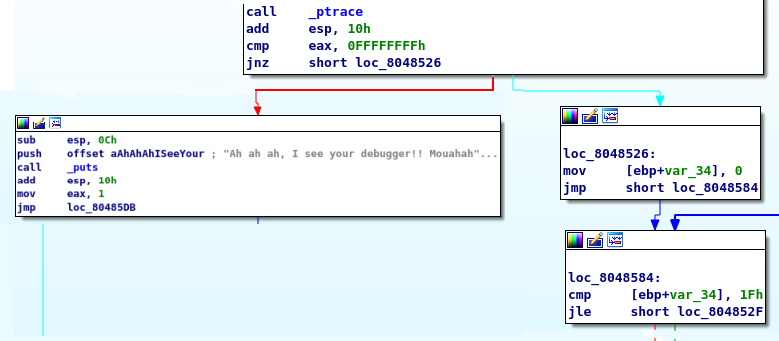
\includegraphics[scale=0.5]{./113-reversing-2-ida-3.PNG}
		\end{center}
	\end{frame}

	\begin{frame}
	\begin{center}
		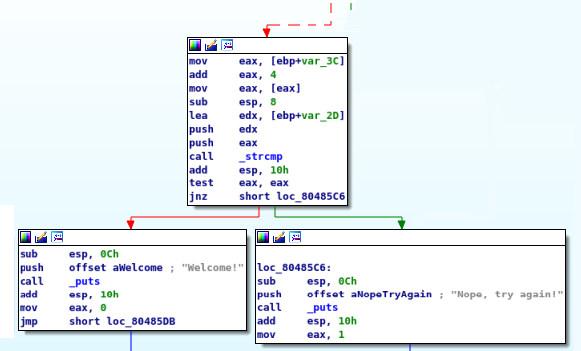
\includegraphics[scale=0.5]{./113-reversing-2-ida-4.PNG}
	\end{center}
	\end{frame}

	\begin{frame}
		\begin{block}{Etape 3}
			\begin{itemize}
				\item Nous allons récupérer les adresses des instructions importantes pour l'attaque. 
				\item Nous allons mettre des points d'arrêt (breakpoints) ainsi que des sauts (jump) pour réussir à voir quelle comparaison (\textbf{strcmp}) fait le programme.
			\end{itemize}
		\end{block}
		\begin{center}
			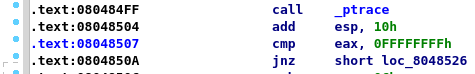
\includegraphics[scale=0.5]{./113-reversing-2-ida-5.PNG}
		\end{center}
			\bigskip
		\begin{center}
			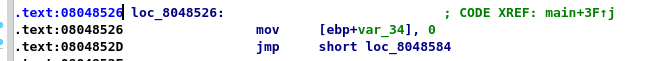
\includegraphics[scale=0.5]{./113-reversing-2-ida-6.PNG}
		\end{center}
			\bigskip
		\begin{center}
			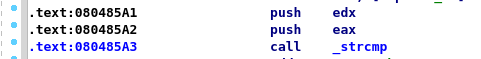
\includegraphics[scale=0.5]{./113-reversing-2-ida-7.PNG}
		\end{center}
	\end{frame}

	\subsection{Détails sur la résolution}
	
	\begin{frame}{Manipulation sur gdb}
		\begin{block}{Etape 3.1}
			\begin{itemize}
				\item \textbf{ptrace()} nous gêne dans la résolution du challenge. En effet, en débuggant, gdb utilise l'appel système \textbf{ptrace}. Le programme testflag le détecte et le quitte immédiatement. \newline
					\tiny{$if (ptrace(PTRACE\_TRACEME, 0, 1, 0) < 0)\{...\}$}
				\normalsize\item Pose d'un breakpoint sur l'adresse du cmp qui fait le branchement du ptrace : $0x08048507$
				\item Jump sur le block qui suit cette comparaison pour être sûr de passer : $0x08048526$
			\end{itemize}
		\end{block}
		\begin{block}{Etape 3.2}
			\begin{itemize}
				\item Pose d'un breakpoint au niveau de l'appel du \textbf{strcmp} : $0x080485a3$
			\end{itemize}
		\end{block}
	\end{frame}

	\begin{frame}{Solution}
		\begin{center}
			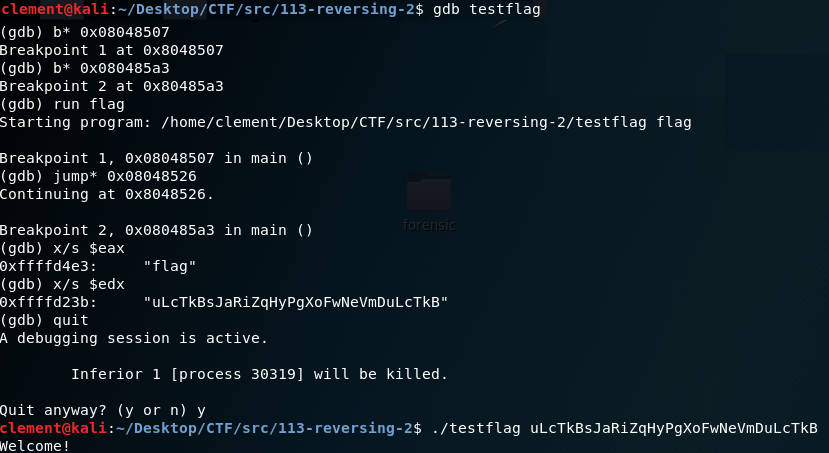
\includegraphics[scale=0.5]{./113-reversing-2-gdb-2.PNG}
		\end{center}
	\end{frame}

	\subsection{Ouverture}

	\begin{frame}
	\begin{block}{Comment éviter cette attaque?}
		\begin{itemize}
		\item Utiliser une fonction de hachage robuste et un salt 
		\item Le programme comparera le hash du salt concaténé au mot de passe de l'utilisateur pour vérifier l'authentification. 
		\end{itemize}
	\end{block}
\end{frame}

      
\end{document}
